\documentclass[a4paper,fleqn,usenatbib]{mnras}

\usepackage{ae, aecompl, amsmath, amssymb}
\usepackage{bm}           %%  bold math
\usepackage{cancel, mathptmx}
\usepackage{color}
\usepackage{dcolumn}  %%  Align table columns on decimal point
\usepackage{epsfig, epsf, etoolbox}
\usepackage{fancyhdr}
\usepackage{graphicx}
\usepackage[T1]{fontenc}
%\usepackage{lscape}
\usepackage{ifthen}
\usepackage{hyperref}
\usepackage{listings}
\usepackage{longtable}
\usepackage{multirow}
\usepackage{newtxtext, newtxmath}
\usepackage{pifont}% http://ctan.org/pkg/pifont
\usepackage{subfigure}
\usepackage{tabu}

\usepackage{verbatim}

\usepackage{xcolor}
%\usepackage[square, sort, comma, numbers]{natbib}
\usepackage{threeparttable}
%\usepackage[square,sort,comma,numbers]{natbib}

\usepackage{graphicx}	% Including figure files
\usepackage{tikz}
\def\checkmark{\tikz\fill[scale=0.4](0,.35) -- (.25,0) -- (1,.7) -- (.25,.15) -- cycle;} 

%%  I dont know why, but arydshln leads to pdflatex crashing (when using 'regular' hline)
%% if you load this package at the top of this list.  e.g. 
%%    tex.stackexchange.com/questions/419497/hline-doesnt-compile-arydshln-and-tabularx-incompatibility
\usepackage{arydshln}


%%%%%%%%%%%%%%%%%%%%%%%%%%%%%%%%%%%%%%%%%%%
%       define Journal abbreviations      %
%%%%%%%%%%%%%%%%%%%%%%%%%%%%%%%%%%%%%%%%%%%
\def\nat{Nat} \def\apjl{ApJ~Lett.} \def\apj{ApJ}
\def\apjs{ApJS} \def\aj{AJ} \def\mnras{MNRAS}
\def\prd{Phys.~Rev.~D} \def\prl{Phys.~Rev.~Lett.}
\def\plb{Phys.~Lett.~B} \def\jhep{JHEP}
\def\npbps{NUC.~Phys.~B~Proc.~Suppl.} \def\prep{Phys.~Rep.}
\def\pasp{PASP} \def\aap{Astron.~\&~Astrophys.} \def\araa{ARA\&A}
\def\jcap{\ref@jnl{J. Cosmology Astropart. Phys.}} 
\def\nar{New~A.R.} 

\newcommand{\preep}[1]{{\tt #1} }

%%%%%%%%%%%%%%%%%%%%%%%%%%%%%%%%%%%%%%%%%%%%%%%%%%%%%
%              define symbols                       %
%%%%%%%%%%%%%%%%%%%%%%%%%%%%%%%%%%%%%%%%%%%%%%%%%%%%%
\def \Mpc {~{\rm Mpc} }
\def \Om {\Omega_0}
\def \Omb {\Omega_{\rm b}}
\def \Omcdm {\Omega_{\rm CDM}}
\def \Omlam {\Omega_{\Lambda}}
\def \Omm {\Omega_{\rm m}}
\def \ho {H_0}
\def \qo {q_0}
\def \lo {\lambda_0}
\def \kms {{\rm ~km~s}^{-1}}
\def \kmsmpc {{\rm ~km~s}^{-1}~{\rm Mpc}^{-1}}
\def \hmpc{~\;h^{-1}~{\rm Mpc}} 
\def \hkpc{\;h^{-1}{\rm kpc}} 
\def \hmpcb{h^{-1}{\rm Mpc}}
\def \dif {{\rm d}}
\def \mlim {m_{\rm l}}
\def \bj {b_{\rm J}}
\def \mb {M_{\rm b_{\rm J}}}
\def \mg {M_{\rm g}}
\def \mi {M_{\rm i}}
\def \qso {_{\rm QSO}}
\def \lrg {_{\rm LRG}}
\def \gal {_{\rm gal}}
\def \xibar {\bar{\xi}}
\def \xis{\xi(s)}
\def \xisp{\xi(\sigma, \pi)}
\def \Xisig{\Xi(\sigma)}
\def \xir{\xi(r)}
\def \max {_{\rm max}}
\def \gsim { \lower .75ex \hbox{$\sim$} \llap{\raise .27ex \hbox{$>$}} }
\def \lsim { \lower .75ex \hbox{$\sim$} \llap{\raise .27ex \hbox{$<$}} }
\def \deg {^{\circ}}
%\def \sqdeg {\rm deg^{-2}}
\def \deltac {\delta_{\rm c}}
\def \mmin {M_{\rm min}}
\def \mbh  {M_{\rm BH}}
\def \mdh  {M_{\rm DH}}
\def \msun {M_{\odot}}
\def \z {_{\rm z}}
\def \edd {_{\rm Edd}}
\def \lin {_{\rm lin}}
\def \nonlin {_{\rm non-lin}}
\def \wrms {\langle w_{\rm z}^2\rangle^{1/2}}
\def \dc {\delta_{\rm c}}
\def \wp {w_{p}(\sigma)}
\def \PwrSp {\mathcal{P}(k)}
\def \DelSq {$\Delta^{2}(k)$}
\def \WMAP {{\it WMAP \,}}
\def \cobe {{\it COBE }}
\def \COBE {{\it COBE \;}}
\def \HST  {{\it HST \,\,}}
\def \Spitzer  {{\it Spitzer \,}}
\def \ATLAS {VST-AA$\Omega$ {\it ATLAS} }
\def \BEST   {{\tt best} }
\def \TARGET {{\tt target} }
\def \TQSO   {{\tt TARGET\_QSO}}
\def \HIZ    {{\tt TARGET\_HIZ}}
\def \FIRST  {{\tt TARGET\_FIRST}}
\def \zc {z_{\rm c}}
\def \zcz {z_{\rm c,0}}


\newcommand{\sqdeg}{deg$^{-2}$}
\newcommand{\lya}{Ly$\alpha$\ }
%\newcommand{\lya}{Ly\,$\alpha$\ }
\newcommand{\lyaf}{Ly\,$\alpha$\ forest}
%\newcommand{\eg}{e.g.~}
%\newcommand{\etal}{et~al.~}
\newcommand{\cii}{C\,{\sc ii}\ }
\newcommand{\ciii}{C\,{\sc iii}]\ }
\newcommand{\civ}{C\,{\sc iv}}
\newcommand{\siiv}{Si\,{\sc iv}\ }
\newcommand{\mgii}{Mg\,{\sc ii}\ }
\newcommand{\feii}{Fe\,{\sc ii}\ }
\newcommand{\feiii}{Fe\,{\sc iii}\ }
\newcommand{\caii}{Ca\,{\sc ii}\ }
\newcommand{\halpha}{H\,$\alpha$\ }
\newcommand{\hbeta}{H\,$\beta$\ }
\newcommand{\oi}{[O\,{\sc i}]\ }
\newcommand{\oii}{[O\,{\sc ii}]\ }
\newcommand{\oiii}{[O\,{\sc iii}]\ }
\newcommand{\heii}{[He\,{\sc ii}]\ }
\newcommand{\nii}{N\,{\sc ii}\ }
\newcommand{\nv}{N\,{\sc v}\ }

%% From:: /cos_pc19a_npr/LaTeX/proposals/JWST/JWST_ERS/Proposal/lines.tex
%%  
\newcommand{\imw}{$i$--$W3$}
\newcommand{\imwf}{$i$--$W4$}
\newcommand{\rmwf}{$r$--$W4$}
\newcommand{\imwt}{$i$--$W2$}
\newcommand{\wtmwf}{$W3$--$W4$}
%\newcommand{\kms}{km s$^{-1}$}
\newcommand{\cmN}{cm$^{-2}$}
\newcommand{\cmn}{cm$^{-3}$}
%\newcommand{\msun}{M$_{\odot}$}
\newcommand{\lsun}{L$_{\odot}$}
\newcommand{\lam}{$\lambda$}
\newcommand{\mum}{$\mu$m}
\newcommand{\ebv}{$E(B$$-$$V)$}
%\newcommand{\heii}{\mbox{He\,{\sc ii}}}
\newcommand{\cv}{\mbox{C\,{\sc v}}}
%\newcommand{\civ}{\mbox{C\,{\sc iv}}}
%\newcommand{\ciii}{\mbox{C\,{\sc iii}}}
%\newcommand{\cii}{\mbox{C\,{\sc ii}}}
%\newcommand{\nv}{\mbox{N\,{\sc v}}}
\newcommand{\niv}{\mbox{N\,{\sc iv}}}
\newcommand{\niii}{\mbox{N\,{\sc iii}}}
%\newcommand{\oi}{\mbox{O\,{\sc i}}}
%\newcommand{\oii}{\mbox{O\,{\sc ii}}}
%\newcommand{\oiii}{\mbox{[O\,{\sc iii}]}}
\newcommand{\oiv}{\mbox{O\,{\sc iv}}}
\newcommand{\ov}{\mbox{O\,{\sc v}}}
\newcommand{\ovi}{\mbox{O\,{\sc vi}}}
\newcommand{\ovii}{\mbox{O\,{\sc vii}}}

%\newcommand{\feii}{\mbox{Fe\,{\sc ii}}}
%\newcommand{\feiii}{\mbox{Fe\,{\sc iii}}}
%\newcommand{\mgii}{\mbox{Mg\,{\sc ii}}}
\newcommand{\neii}{[Ne\,{\sc ii}]\ }
\newcommand{\neiii}{[Ne\,{\sc ii}]\ }
\newcommand{\nev}{Ne\,{\sc v}\ }
\newcommand{\nevi}{[Ne\,{\sc vi}]\ }
\newcommand{\neviii}{\mbox{Ne\,{\sc viii}}}
\newcommand{\aliii}{\mbox{Al\,{\sc iii}}}
\newcommand{\siii}{\mbox{Si\,{\sc ii}}}
\newcommand{\siiii}{\mbox{Si\,{\sc iii}}}
%\newcommand{\siiv}{\mbox{Si\,{\sc iv}}}
%\newcommand{\lya}{\mbox{Ly$\alpha$}}
%\newcommand{\lyb}{\mbox{Ly$\beta$}}
\newcommand{\hi}{\mbox{H\,{\sc i}}}
\newcommand{\snine}{\mbox{[S\,{\sc ix}]}}
\newcommand{\sivi}{\mbox{[Si\,{\sc vi}]}}
\newcommand{\sivii}{\mbox[{Si\,{\sc vii}]}}
\newcommand{\siix}{\mbox{[Si\,{\sc ix}]}}
\newcommand{\six}{\mbox{[Si\,{\sc x}]}}
\newcommand{\sixi}{\mbox{[Si\,{\sc xi}]}}
\newcommand{\caviii}{\mbox{[Ca\,{\sc viii}]}}
\newcommand{\arii}{\mbox{[Ar\,{\sc ii}]}}

%%[Ar II] 6.97
%% [S IX] 1.252 μm 328 
% [Si X] 1.430 μm 351 
% [Si XI] 1.932 μm 401 
% [Si VI] 1.962 μm 167 
% [Ca VIII] 2.321 μm 128 
% [Si VII] 2.483 μm 205 
% [Si IX] 3.935 μm 303
% [Ar II] 6.97


%\snine\ at 1.252$\mu$m, \six\ at 1.430$\mu$m, \sixi\ at 1.932$\mu$m, \sivi\ at
%1.962$\mu$m, \caviii\ at 2.321$\mu$m, \sivi\ at 2.483$\mu$m \siix\ at
%3.935$\mu$m and \arii\ at 6.97$\mu$m. 
%%
%% such as [Ne ii]12.8 μm, [Ne v]14.3 μm, [Ne iii]15.5 μm, [S iii]18.7 μm and 33.48 μm, [O iv]25.89 μm and [Si ii]34.8 μm (e.g
%%
%% MIR emission lines like [NeII] and [NeV] are ..
%%
%% Also,  arXiv:astro-ph/0003457v1 
%% [NeV] 14.32um & 24.32um and [NeVI] 7.65um imply an A(V)>160 towards the NLR...
%% [NeIII]15.56um/[NeII]12.81um
%%
%% [Ne V] 14.3, 24.2 μm 97.
%% [Ne II] 12.8 μm
%% [OIV] 26μm
%%


%%%%%%%%%%%%%%%%%%%%%%%%%%%%%%%%%%%%%%%%%%%%%%%%%%%%%
%              define Listings                       %
%%%%%%%%%%%%%%%%%%%%%%%%%%%%%%%%%%%%%%%%%%%%%%%%%%%%%
\definecolor{dkgreen}{rgb}{0,0.6,0}
\definecolor{gray}{rgb}{0.5,0.5,0.5}
\definecolor{mauve}{rgb}{0.58,0,0.82}

\lstset{frame=tb,
  language=Python,
  aboveskip=3mm,
  belowskip=3mm,
  showstringspaces=false,
  columns=flexible,
  basicstyle={\small\ttfamily},
  numbers=none,
  numberstyle=\tiny\color{gray},
  keywordstyle=\color{blue},
  commentstyle=\color{dkgreen},
  stringstyle=\color{mauve},
  breaklines=true,
  breakatwhitespace=true,
  tabsize=3
}



\title[High-redshift CLQs]{The first high-redshift Changing Look Quasars}

\author[Bercow]
{The RH John~S.~Bercow, MP, {\it et al.} 
%Nicholas~P.~Ross$^{1}$\thanks{E-mail: npross@roe.ac.uk},    
%K. E. Saavik Ford$^{2,3,4}$,  Matthew Graham$^{5}$,  Barry McKernan$^{2,3,4}$,  
%\newauthor Daniel Stern$^{6}$, 
%Aaron M. Meisner$^{7,8}$, Roberto J. Assef$^{9}$, Arjun Dey$^{10}$, Andrew J. Drake$^{11}$, \newauthor Hyunsung D. Jun$^{12}$, Dustin Lang$^{13,14,15}
\\
% List of institutions
$^{1}$Speaker's Chair, The House of Commons, London, SW1A 0AA \\
%$^{1}$Institute for Astronomy, University of Edinburgh, Royal Observatory, Blackford Hill, Edinburgh EH9 3HJ, United Kingdom \\
%$^{2}$Department of Science, BMCC, City University of New York, New York, NY 10007, USA \\
%$^{3}$Department of Astrophysics, Rose Center for Earth and Space, American Museum of Natural History, Central Park West at 79th Street, NY 10024, USA \\
%$^{4}$Graduate Center, City University of New York, 365 5th Avenue, New York, NY 10016, USA\\
%$^{5}$Cahill Center for Astronomy and Astrophysics, California Institute of Technology, Mail Code 249/17, 1200 E California Blvd, Pasadena CA 91125, USA\\
%$^{6}$Jet Propulsion Laboratory, California Institute of Technology, 4800 Oak Grove Drive, Mail Stop 169-221, Pasadena, CA 91109, USA \\
}

\date{Accepted XXX. Received YYY; in original form ZZZ}
\pubyear{2018}

%\hypersetup{draft}
\begin{document}
\label{firstpage}
\pagerange{\pageref{firstpage}--\pageref{lastpage}}
\maketitle


\begin{abstract}
This is two hundred words, the suggested maximum for a MNRAS
Letter. Lorem ipsum dolor sit amet, autem semper eam ei. Eros
maluisset posidonium eu mea, atqui aperiam nostrum cum ad. Te vocent
volutpat petentium vix, pro senserit convenire vituperatoribus ex, ad
his mucius tamquam appetere. An mea omnium voluptaria scribentur, te
verear iisque vulputate sit. Vim malis omittam probatus cu, vide
tempor ius ex, vim eu case magna rebum. Vis id clita eruditi, in sea
evertitur dissentiunt, per eu deseruisse mnesarchum deterruisset. Eu
tale tempor sea, te mundi congue detracto est. Has ipsum animal timeam
no. Atqui novum nobis et his, pericula interesset mel ut. Ea pro eros
everti legendos. Vel iusto legere euismod id, ea erat debitis
democritum usu. Ut paulo aliquid vix, disputationi delicatissimi
signiferumque ut eam. Utroque impedit ad his. Ei mea sale tritani, ex
eum duis epicuri, at per nonumy delectus electram. Dolorem patrioque
prodesset vis at, sint tritani mel te. Ut nulla solet nonumes has, mel
diam scripta delectus in, ne duo laudem appetere assueverit. An vim
reque munere, labores apeirian his cu. Ei clita placerat praesent nam,
in affert sapientem est. Qui te regione deterruisset. Nam at quodsi
placerat. Pri no quando placerat.
\end{abstract}

% Select between one and six entries from the list of approved keywords.
% Don't make up new ones.
\begin{keywords}
accretion, accretion discs -- surveys -- quasars: general -- quasars: individual: J1100-0053 
\end{keywords}



%%%%%%%%%%%%%%%%%%%%%%%%%%%%%%%%%%%%%%%%%%%%%%%%%%%%%%%%%%%%%%%%%%%%%%%%%%%%%%%%%
%%%%%%%%%%%%%%%%%%%%%%%%%%%%%%%%%%%%%%%%%%%%%%%%%%%%%%%%%%%%%%%%%%%%%%%%%%%%%%%%%
%%
%%
%%   SECTION 1  SECTION 1  SECTION 1  SECTION 1  SECTION 1  SECTION 1  
%%   SECTION 1  SECTION 1  SECTION 1  SECTION 1  SECTION 1  SECTION 1  
%%   SECTION 1  SECTION 1  SECTION 1  SECTION 1  SECTION 1  SECTION 1  
%%
%%
%%%%%%%%%%%%%%%%%%%%%%%%%%%%%%%%%%%%%%%%%%%%%%%%%%%%%%%%%%%%%%%%%%%%%%%%%%%%%%%%%%
%%%%%%%%%%%%%%%%%%%%%%%%%%%%%%%%%%%%%%%%%%%%%%%%%%%%%%%%%%%%%%%%%%%%%%%%%%%%%%%%%%
\section{Introduction}
Luminous AGN, i.e. quasars, are now seen to significantly vary their
energy output on timescales of weeks to months.  This observation, and
the subsequent mismatch in the expected ``viscous'' timescale, which
for a $\approx$10$^{7}$ M$_{\odot}$ is $\sim$hundreds of years, was
noted over 30 years ago \citep[e.g.][]{Alloin1985}. However, with new
photometric light-curve and repeat spectroscopic data, the desire for
a deeper understanding of AGN accretion disk physics has been recently
re-invigorated the field \citep[e.g.][]{Lawrence2018, Antonucci2018}.

Samples of over 100 ``Changing Look'' quasars (CLQs) or ``Changing
State'' quasars (CSQs) have now been assembled
\citep[e.g.][]{MacLeod2019, Graham2019}. The community uses both these
terms as a cover for the underlying physics. For sake of argument,
``Changing Look'' quasars can be thought of as the extension of
``regular'' quasar variability \citep[e.g.][]{MacLeod2012} whereas the
``Changing State'' quasars (CSQs) have a `state-transition' similar to
that in Galactic X-ray binaries \citep[e.g][]{NodaDone2018, Ruan2019}.
These CLQs have primarily been defined according to the
(recombination) Balmer emission line properties with particular
attention paid to the H$\beta$ emission line, usually observed from
optical spectroscopy.  As such, current CLQ studies have been at
redshifts $z<1$.

While there have been a slew of studies on triply ionized carbon, i.e
\civ, these have tended to focus on broad absorption line quasars
\citep[BAL QSOs; see e.g. Table 1][]{Hemler2019} or the Baldwin Effect
\citep[BEff; e.g. ][]{Baldwin1977, Bian2012, Jensen2016,
Hamann2017}\footnote{As noted in \citet{Rakic2017}, two different
types of Baldwin effect are present in the literature: the {\it
global} (or {\it ensemble}) Baldwin Effect, which is an
anti-correlation between the EW of the emission line and the
underlying continuum luminosity of {\it single-epoch} observations of
a {\it large number} of AGN and second, the {\it intrinsic} Baldwin
effect, the same anti-correlation but in an {\it individual, variable}
AGN \citep{PoggePeterson1992}.}.  Dramatic changes in the
collisionally excited broad {\it emission} line (BEL) of \civ (and
indeed \ciii) have not to this point been seen.

Here, we report on three quasars  
%SDSS J120544.7+342252.4  (hereafter J1205+3422), 
%SDSS J163852.93+282707.7 (hereafter J1638+2827) and
%SDSS J222818.76+220102.9 (hereafter J2228+2201)  
which show dramatic changes in their \civ\ and \ciii broad emission
line properties as well as in the underlying continuum. We claim these
are the first examples of ``Changing Look Quasars'' at high ($z>1$)
redshift. Moreover, these are the first cases for substantial changes
of ions with high ionization potentials (I.P.'s $>$2 Rydberg), thus
linking the ionizing photons to the energetic inner accretion disk,
potentially by inverse Compton scattering lower energy photons to
higher energies.  Furthermore, the measured rest-wavelengths of
emission lines in quasar spectra, are known to vary from their nominal
laboratory especially for the high-ionization broad lines,
wavelengths, \citep[e.g.][]{VandenBerk2001}.

In this paper we use the wavelengths of 1548.202 and 1550.774 \AA\ for
the \civ doublet \citep{Kramida2018}.
%%  The singly ionized hydrogen atom H+ is referred to as HII, doubly ionized oxygen O++ is called OIII, etc.
%%  “24.4 eV is energy needed for C I to get rid of two electrons, and become doubly-ionised C III”
%%  https://en.wikipedia.org/wiki/Ionization_energies_of_the_elements_(data_page)
The ground state of carbon is 1$s^2$ 2$s^2$ 2$p^2$.  Using the
\href{https://physics.nist.gov/PhysRefData/ASD/ionEnergy.html}{NIST
Atomic Spectra Database Ionization Energies Form} for ionisation
energies, we see 11.3 eV is the energy needed for C I to dislodge one
electron and become singly-ionised C II; 24.4 eV is energy needed for
singly-ionised C II to dislodge an additional electron, and become
doubly-ionised C III, and 47.89 eV (3.519 Ry) is required for
doubly-ionised C III become triply--ionised \civ.  64.49 eV (4.74 Ry)
is the energy needed to ionize \civ itself.
%%
The 1548.202 and 1550.774 \AA\ emission doublet is created by the 2$p$
$^{2}P_{0}$ $---$ 2$s$ $^{2}S$ transition with energies 64,484
cm$^{-1}$ and 64591 cm$^{-1}$ \citep[e.g.][]{Moore1993}.
%Ground  Shells:  1$s^{2}$2$s$. 
%Ground  Level: $^{2}S_{1/2}$. 
%Ionized  Level: 1$s^{2}$ $^{1}S_{0}$. 
 
%%\subsection{Literature Search}
\civ\ variability has been long studied, \citep[e.g., ][]{Baldwin1977,
Gaskell1982, Gregory1982, Wilkes1986, Espey1989, Espey1990Erratum,
ZhengSulentic1990, Corbin1990, Corbin1991, Weymann1991,
Dimitrijevic1992, TytlerFan1992, Wills1993, Brotherton1994, Osmer1994,
Laor1995, McIntosh1999}.
%%
%\citet{Gregory1982} reported time variability in both Lya and \civ 1550 emission lines in the Seyfert galaxy NGC 5548.
%
%\citet{1994}
%\includegraphics[]{../../../../../Users/npr1/Downloads/1994ASPC___69____1P.pdf}

%% NAZAROVA 2003
%% BROAD EMISSION LINES La, C IV AND Hb IN NGC 5548
%% Astronomical and Astrophysical Transactions
%% Vol. 22, Nos. 4–5, August–October 2003, pp. 681–689
\citep{Nazarova2003} ...

\citet{Wilhite2006} examine the variability of a C~\textsc{iv} 
sample of 105 quasars observed at multiple epochs by the SDSS. 
They find a strong correlation between the change in the C~\textsc{iv} line flux and the
change in the line width, but no correlations between the change in 
flux and changes in line center and skewness.  These authors find 
that the relation between line flux change and line width change is consistent with a model in
which a broad line base varies with greater amplitude than the line
core. The C~\textsc{iv} lines in these 
high-luminosity quasars appear to be less responsive to continuum
variations than those in lower luminosity AGN.  
%% Additionally, we find no evidence for variability of the well known
blueshift of the C~\textsc{iv} line with respect to the low-ionization
Mg~\textsc{ii}$\lambda$2798 line in the highest flux objects,
indicating that this blueshift might be useful as a measure of
orientation.

%% Punsly 2010
%% Astrophysical Journal, 713, 232
%% THE REDSHIFTED EXCESS IN QUASAR C iv BROAD EMISSION LINES

\citet{Richards2011} explored the BELR in over 30,000 $z > 1.54$ SDSS
quasars, concentrating on the properties of the \civ\ emission
line. We consider two well-known effects involving the \civ\ emission
line: the anti-correlation between the \civ\ EQW and luminosity (i.e.,
the BEff) and the blueshifting of the peak of \civ\ emission with
respect to the systemic redshift. These authors conclude that these
two \civ\ parameters (EQW and blueshift) are capturing an important
trade-off between ``disk'' and ``wind'' components in the disk-wind
model of accretion disks \citep[e.g.,][]{Murray1995, Elvis2000, Proga2000}.  with one dominating over the other depending on the
shape of the SED \citep[][]{Leighly2004b}.  (strong \civ EQW indicates
a more ionizing SED and large \civ blueshift indicating a less
ionizing SED).

%% \citet{Grier2015}....
%% \includegraphics[]{../../../../../Users/npr1/Downloads/Grier_2015_ApJ_806_111.pdf}
%% \citet{Denney2015}, 
%%Denney, Kelly; SDSS-RM Team, ``The Effects of S/N on Measuring CIV Broad Emission Line Widths in Quasars - An Early Science Result from the Sloan Digital Sky Survey Reverberation Mapping Project'' ; http://adsabs.harvard.edu/abs/2015AAS...22520403D
The Sloan Digital Sky Survey Reverberation Mapping (SDSS-RM) Project 
\citep{Shen2015} has a  monitored $\sim$350 quasars with \civ
Noting the biases associated with \civ Emission Line Properties 
\citep[e.g. increasing systematic offsets with decreasing signal-to-noise][]{Denney2016}, 
\citet{Grier2019} report 
report significant time delays between the continuum and the CIV 1549 emission line in 52 quasars, 
and investigate the \civ radius-luminosity relationship. 

%% \citet{Coatman2017} 
%The \civ $\lambda \lambda$1498,1501 broad emission line is visible in optical spectra to redshifts exceeding $z\sim5$. 
\civ has long been known to exhibit significant displacements to the blue and these `blueshifts' almost certainly signal the presence of strong outflows. As a consequence, single-epoch virial black hole (BH) mass estimates derived from \civ velocity widths are known to be systematically biased compared to masses from the hydrogen Balmer lines. 
\citet{Coatman2017} use a large sample of 230 high-luminosity (LBol = 1045.5-1048 erg s-1), redshift $1.5 < z < 4.0$ quasars with both \civ and Balmer line spectra, we have quantified the bias in \civ BH masses as a function of the \civ blueshift. \civ BH masses are shown to be a factor of 5 larger than the corresponding Balmer-line masses at C IV blueshifts of 3000 km s$^{-1}1$ and are overestimated by almost an order of magnitude at the most extreme blueshifts, $\gtrsim$5000 km s$^{-1}$. 
%Using the monotonically increasing relationship between the \civ blueshift and the mass ratio BH(\civ)/BH(H$\alpha$), we derive an empirical correction to all C IV BH masses. The scatter between the corrected C IV masses and the Balmer masses is 0.24 dex at low C IV blueshifts ($\sim$0 km s-1) and just 0.10 dex at high blueshifts ($\sim$3000 km s$^{-1}$), compared to 0.40 dex before the correction. The correction depends only on the C IV line properties - i.e. full width at half-maximum and blueshift - and can therefore be applied to all quasars where C IV emission line properties have been measured, enabling the derivation of unbiased virial BH-mass estimates for the majority of high-luminosity, high-redshift, spectroscopically confirmed quasars in the literature.

\citet{Sun2018} use the multi-epoch spectra of 362 quasars from the Sloan Digital Sky Survey Reverberation Mapping project to investigate the dependence of the blueshift of \civ relative to \mgii on quasar properties. We confirm that high-blueshift sources tend to have low \civ equivalent widths (EWs), and that the low-EW sources span a range of blueshift. Other high-ionization lines, such as He II, also show similar blueshift properties. The ratio of the line width (measured as both the full width at half maximum and the velocity dispersion) of \civ to that of \mgii increases with blueshift. Quasar variability enhances the connection between the \civ blueshift and quasar properties (e.g., EW). The variability of the \mgii line center (i.e., the wavelength that bisects the cumulative line flux) increases with blueshift. In contrast, the C IV line center shows weaker variability at the extreme blueshifts. Quasars with the high-blueshift \civ lines tend to have less variable continuum emission, when controlling for EW, luminosity, and redshift. Our results support the scenario that high-blueshift sources tend to have large Eddington ratios.
%%
Therefore, the \civ\ or \heii\ EW is not an accurate indicator of the Eddington ratio or quasar SED.
%%
Recent investigations also include \citet{Meyer2019}. 

This paper is organised as follows. In Section 2, we describe our
sample selection, catalogs and observationa data sets.  In Section 3,
we present various theoretical models and discuss if and how each
describes and explains the data.  We conclude in Section 4.  We report
all magnitudes on the AB zero-point system \citep{Oke_Gunn1983,
Fukugita1996} unless otherwise stated explicitly. For the WISE bands,
$m_{\rm AB} = m_{\rm Vega} + m$ where $m = (2.699, 3.339)$ for WISE W1
at 3.4$\mu$m and WISE W2 at 4.6$\mu$m, respectively
\citep{Cutri2011}. We choose the cosmological parameters
$\Omega_{\Lambda} = 0.7$, $\Omega_{\rm M} = 0.3$, and $h = 0.7$ in
order to be consistent with \citet{Shen2011}.


%%%%%%%%%%%%%%%%%%%%%%%%%%%%%%%%%%%%%%%%%%%%%%%%%%%%%%%%%%%%%%%%%%%%%%%%%%%%%
%%%%%%%%%%%%%%%%%%%%%%%%%%%%%%%%%%%%%%%%%%%%%%%%%%%%%%%%%%%%%%%%%%%%%%%%%%%%%
%%
%%   SECTION 2   SECTION 2   SECTION 2   SECTION 2   SECTION 2   SECTION 2  
%%   SECTION 2   SECTION 2   SECTION 2   SECTION 2   SECTION 2   SECTION 2  
%%   SECTION 2   SECTION 2   SECTION 2   SECTION 2   SECTION 2   SECTION 2  
%%
%%%%%%%%%%%%%%%%%%%%%%%%%%%%%%%%%%%%%%%%%%%%%%%%%%%%%%%%%%%%%%%%%%%%%%%%%%%%%
%%%%%%%%%%%%%%%%%%%%%%%%%%%%%%%%%%%%%%%%%%%%%%%%%%%%%%%%%%%%%%%%%%%%%%%%%%%%%
\section{Data}
%\subsection{Selection/Identification}
\subsection{Spectra}
An overview of our spectroscopic observations is given in Table~\ref{tab:obs_notes}. 
The spectra are from the SDSS \citep{Stoughton2002, DR7, Schneider2010},  
the SDSS-III Baryon Oscillation Spectroscopic Survey \citep[BOSS][]{Eisenstein2011, Dawson2013, Smee2013, Alam2015, Paris2017} 
and the SDSS-IV  Extended Baryon Oscillation Spectroscopic Survey \citep[eBOSS; ][]{Dawson2016, Abolfathi2018}. 
These quasars were targetted via a range of techniques and algorithms \citep[][]{Richards2002, Ross2012, 
Myers2015}.  
These data are supplemented by spectra from 
the Low Resolution Imaging Spectrometer (LRIS) on the 10m Keck {\sc I} telescope \citep{Oke1995}. 
%% The Keck Low Resolution Imaging Spectrometer", Oke, J.B., et al.. 1995, PASP, 107, 375
and the Double Spectrograph (DBSP) instrument on the Palomar {\it Hale} 5m telescope. 


\subsection{Line Properties}. 
We use the measured quasar emission line properties from \citet{Shen2011} and \citet{Hamann2017}. 
\citet{Hamann2017} in particular investigate in robust detail the UV continuum and the \civ (and \nv $\lambda$ $\lambda$1238, 1242) emission lines in 
over 200,000 quasars in BOSS DR12Q \citep{Paris2017}\footnote{This emission-line catalog 
can be downloaded from \href{https://datadryad.org/stash/dataset/doi:10.6086/D1H59V}{here}.}
The quasar redshift are limited to the range 1.53 ≤ ze ≤ 5.0 so that C IV and the adjacent continuum are covered by BOSS. 
These measurements provide line profile information and N V/C IV flux ratios 

Sed elit massa, eleifend non sodales a, commodo ut felis. Sed id
pretium felis. Vestibulum et turpis vitae quam aliquam convallis. Sed
id ligula eu nulla ultrices tempus. Phasellus mattis erat quis metus
dignissim malesuada. Nulla tincidunt quam volutpat nibh facilisis
euismod. Cras vel auctor neque. Nam quis diam risus.

\begin{table}
 \centering
 \begin{tabular}{l l l l}
  \hline \hline 
% &&\\
   Quantity \ Object                           & J2228+2201     &  J1638+2827 \\
% &&\\
 \hline 
    &&\\
    R.A. / deg                                        &    337.078194      &  249.720559\\
    Declination / deg                            &    +22.017478      &  +28.452159 \\
    redshift, $z$                                    &   2.222$\pm$0.00038   &  2.185$\pm$0.00043          \\
    &&\\ 
    \multirow{2}{*}{Plate, Fiber, MJD}   & 6118, 720, 56189	     &  2948, 614, 54553	  \\
                                         & 7582, 790, 56960	     & 5201, 178, 55832 \\    
 %   &&\\ 
    %$M_{i}(z=2)$  / mag                          &   ?                       & ?                \\
    %log $(L_{\rm bol} / {\rm erg s}^{-1}) $      &   ?             & 45.56$\pm$0.004      & 45.07$\pm$0.004 \\
    %log $(M_{\rm BH} / M_{\odot})  $           &  ?                  & 8.43$\pm$0.03           & 8.46$\pm$0.02 \\
    %Eddington ratio  (\%)                        &  ?                               &  10.7                           &  3.2     \\ 
    &&\\
    \hline \hline 
  \end{tabular}
  \caption{Physical properties of J1100-0053, J2317+0005 and J1052+1519 using the
    methods from \citet{Shen2011}. *This spectrum was used to estimate
    the quantities reported.  We use the regular definition of $L_{\rm
      Edd} = 4 \pi G M m_{\rm p} c /\sigma_{T} =
    1.26\times10^{38}\left (M/M_{\odot} \right )$ erg s$^{-1}$.} 
 \label{tab:Shen_props}
\end{table}



\begin{table*}
 \centering
 \begin{tabular}{r  r  r r r   r r r r}
  \hline \hline 
% &&\\
   Object                         & \multirow{3}{*}{Redshift} & \multirow{3}{*}{Mag}      & \multirow{3}{*}{MJD} & \multirow{3}{*}{Date}  & \multirow{3}{*}{Instrument}   & Exposure    & \multirow{3}{*}{Spectrum} & \multirow{3}{*}{Notes} \\
   R.A. / deg                   &               &               &            &                                &                                                                       &  Time         & & \\
   Decl. / deg                 &               &               &            &                                &                                                                       &  / seconds         & & \\

% &&\\
 \hline 
                                       &                &               &            &                              &                   &                             &  & \\
   J120544.7+342252.4   & 2.071     &   17.99   & 53498 & 2005-May-08   & SDSS             & ?                          & 53498-2089-427  & \\
          181.436164           &                &               & 58538 & 2019-Feb-24     & DBSP            &  2$\times$900    &                               &  Conditions? \\
         +34.381229           &                &               & 58693 & 2019-Jul-29      & DBSP            &  2$\times$1200   &                                &   \\
                                       &                &               &              &                           &                   &                             &  & \\
   J163852.9+282707.7   & 2.182     &   19.77    & 54553 & 2008-Mar-28    & SDSS             & ?                          & 54553-2948-614  & \\
      249.720558407	       &               &              & 55832  & 2011-Sep-28     & BOSS            &   3603                  & 55832-5201-178  & \\
       +28.452158884        &               &              & 58583 & 2019-Apr-10        & LRIS              &  2$\times$900    &   & \\
                                       &                &               &              &                           &                   &                             &  & \\
    J222818.7+220102.9   & 2.222     & 19.97    & 56189 & 2012-Sep-19     & BOSS             &  2702               & 56189-6118-720   & \\
        337.078194              &              &              & 56960 & 2014-Oct-30    & BOSS             & ?                         & 56960-7582-790     & QSO1-REOBS \\ 
        +22.017478                                &               &             & 58693 & 2019-Jul-29      & DBSP              & 2$\times$1200  &       &    \\
                                       &                &               &            &                             &                   &                              &  & \\
%   J232446.7+140029.5   &  0.916     &  18.83   &  56209 & 2012-Oct-09   & BOSS             & ?                             & 56209-6148-743   & \\
 %                                      &                &               &   58662 & 2019-Jun-28  &   (??)DBSP       & ?                            &  & \\
  %                                     &                &               &              &                           &                   &                              &  & \\
   \hline \hline   
  \end{tabular}
  \caption{Spectrum is SDSS/BOSS MJD-Plate-FiberID combination. 
Exposure times are from the {\tt plate.fits} file. 
DBSP on the Palomar 200-inch telescope is the } 
 \label{tab:obs_notes}
\end{table*}



\subsection{Multi-wavelength properties}
MIR \\
Radio \\
{\bf FROM ROSS ET AL 2018!!!!} 
While previous efforts have used the 1-year baseline of the WISE mission to identify
changing-look quasars \citep[e.g.,][]{Assef2018, Stern2018}, our
investigation is the first to extend this selection to the infrared
using NEOWISE-R mission data. We have identified a sample of Sloan
Digital Sky Survey (SDSS) quasars that show significant changes in
their IR flux over the course of a few years. Importantly, our IR
light curves enable us to set limits on SED changes due to
obscuration.

We use data from the
beginning of the WISE mission \citep[2010 January; ][]{Wright2010}
through the thrid-year of NEOWISE-R operations \citep[2016 December;
][]{Mainzer2011}. The WISE scan pattern leads to coverage of the
full-sky approximately once every six months (a ``sky pass''), but the
satellite was placed in hibernation in 2011 February and then
reactivated in 2013 October. Hence, our light curves have a cadence of
6 months with a 32 month sampling gap.

The W1/W2 light curves for $\sim$200,000 SDSS and BOSS spectroscopic
quasars were obtained by performing forced photometry at the locations
of DECam-detected optical sources \citep{Lang2014, Meisner2017a,
Meisner2017b}. This forced photometry was performed on time-resolved
coadds \citep{Lang2014}, each of which represents a stack of $\sim$12
exposures. The coaddition removes the possibility of probing
variability on $\lesssim$1 day time scales, but pushes $\approx$1.4
magnitudes deeper than individual exposures while removing virtually
all single-exposure artifacts (e.g. cosmic rays and satellites).

Approximately $\sim$30,000 of the SDSS/BOSS quasars with W1/W2
light-curves available are `IR-bright', in that they are above both
the W1 and W2 single exposure thresholds and therefore detected at
very high significance in the coadds. For this ensemble of objects,
the typical variation in each quasar's measured (W1-W2) color is 0.06
magnitudes.  This includes statistical and systematic errors which are
expected to contribute variations at the few hundredths of a magnitude
level. The typical measured single-band scatter is 0.07 magnitudes in
each of W1 and W2.



%%\newpage
%% For the MNRAS Letter, not sure this can take up a full page...
\begin{figure}
  \centering
  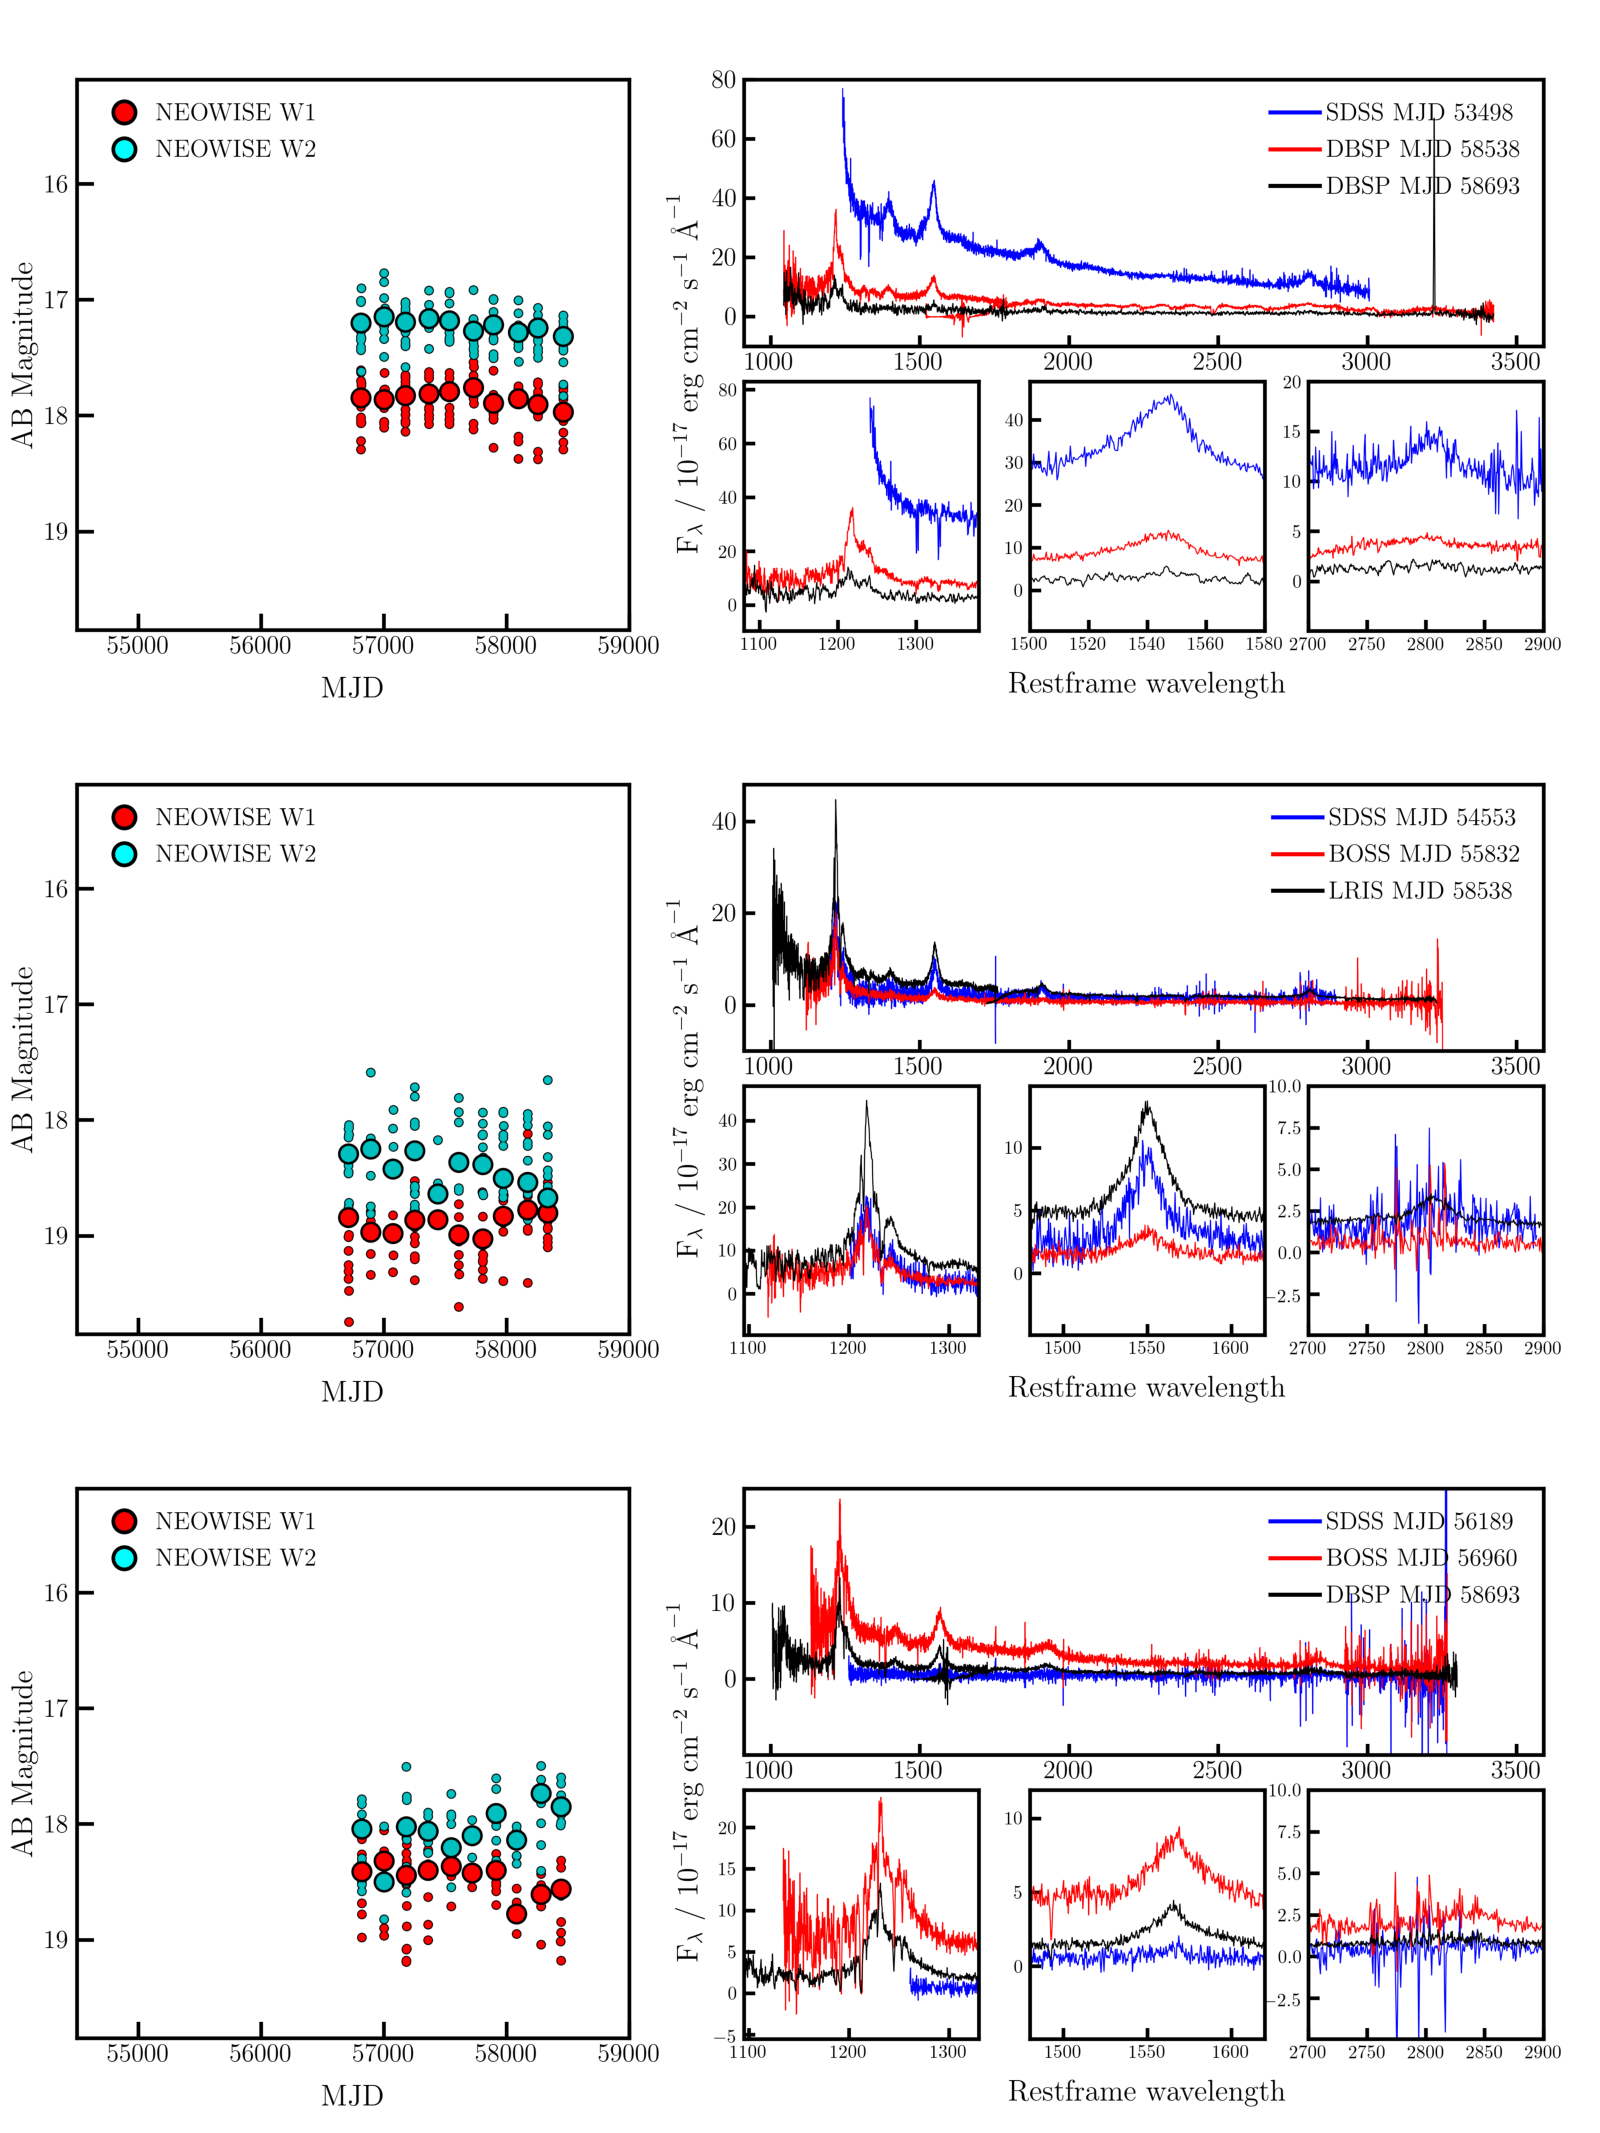
\includegraphics[width=8.7cm, trim=0.2cm 0.2cm 0.2cm 0.2cm, clip]
  {../plots/spectral/The_3_CIV_CLQs_20190917.pdf}
% {figures/The_3_CIV_CLQs_20190917.pdf}
   \vspace{-12pt}
  \caption[]{The threes high-$z$ CLQ quasars; 
SDSS J1205+3422 (top), 
SDSS J1638+2827 (middle), 
SDSS J2228+2201 (bottom). 
%A quasar at $z = 2.2$ with the two spectra showing CIV and CIII] fading.
}
  \label{fig:civ_clqs}
\end{figure}

\begin{figure*}
  \centering
  %% trim=l b r t
  \includegraphics[width=16.7cm, trim=0.0cm 0.1cm 0.2cm 0.1cm, clip]
  % {../plots/spectral/The_3_CIV_CLQs_20190917.pdf}
  {../plots/perObject/J1205+3422_landscape_20190920.png}
  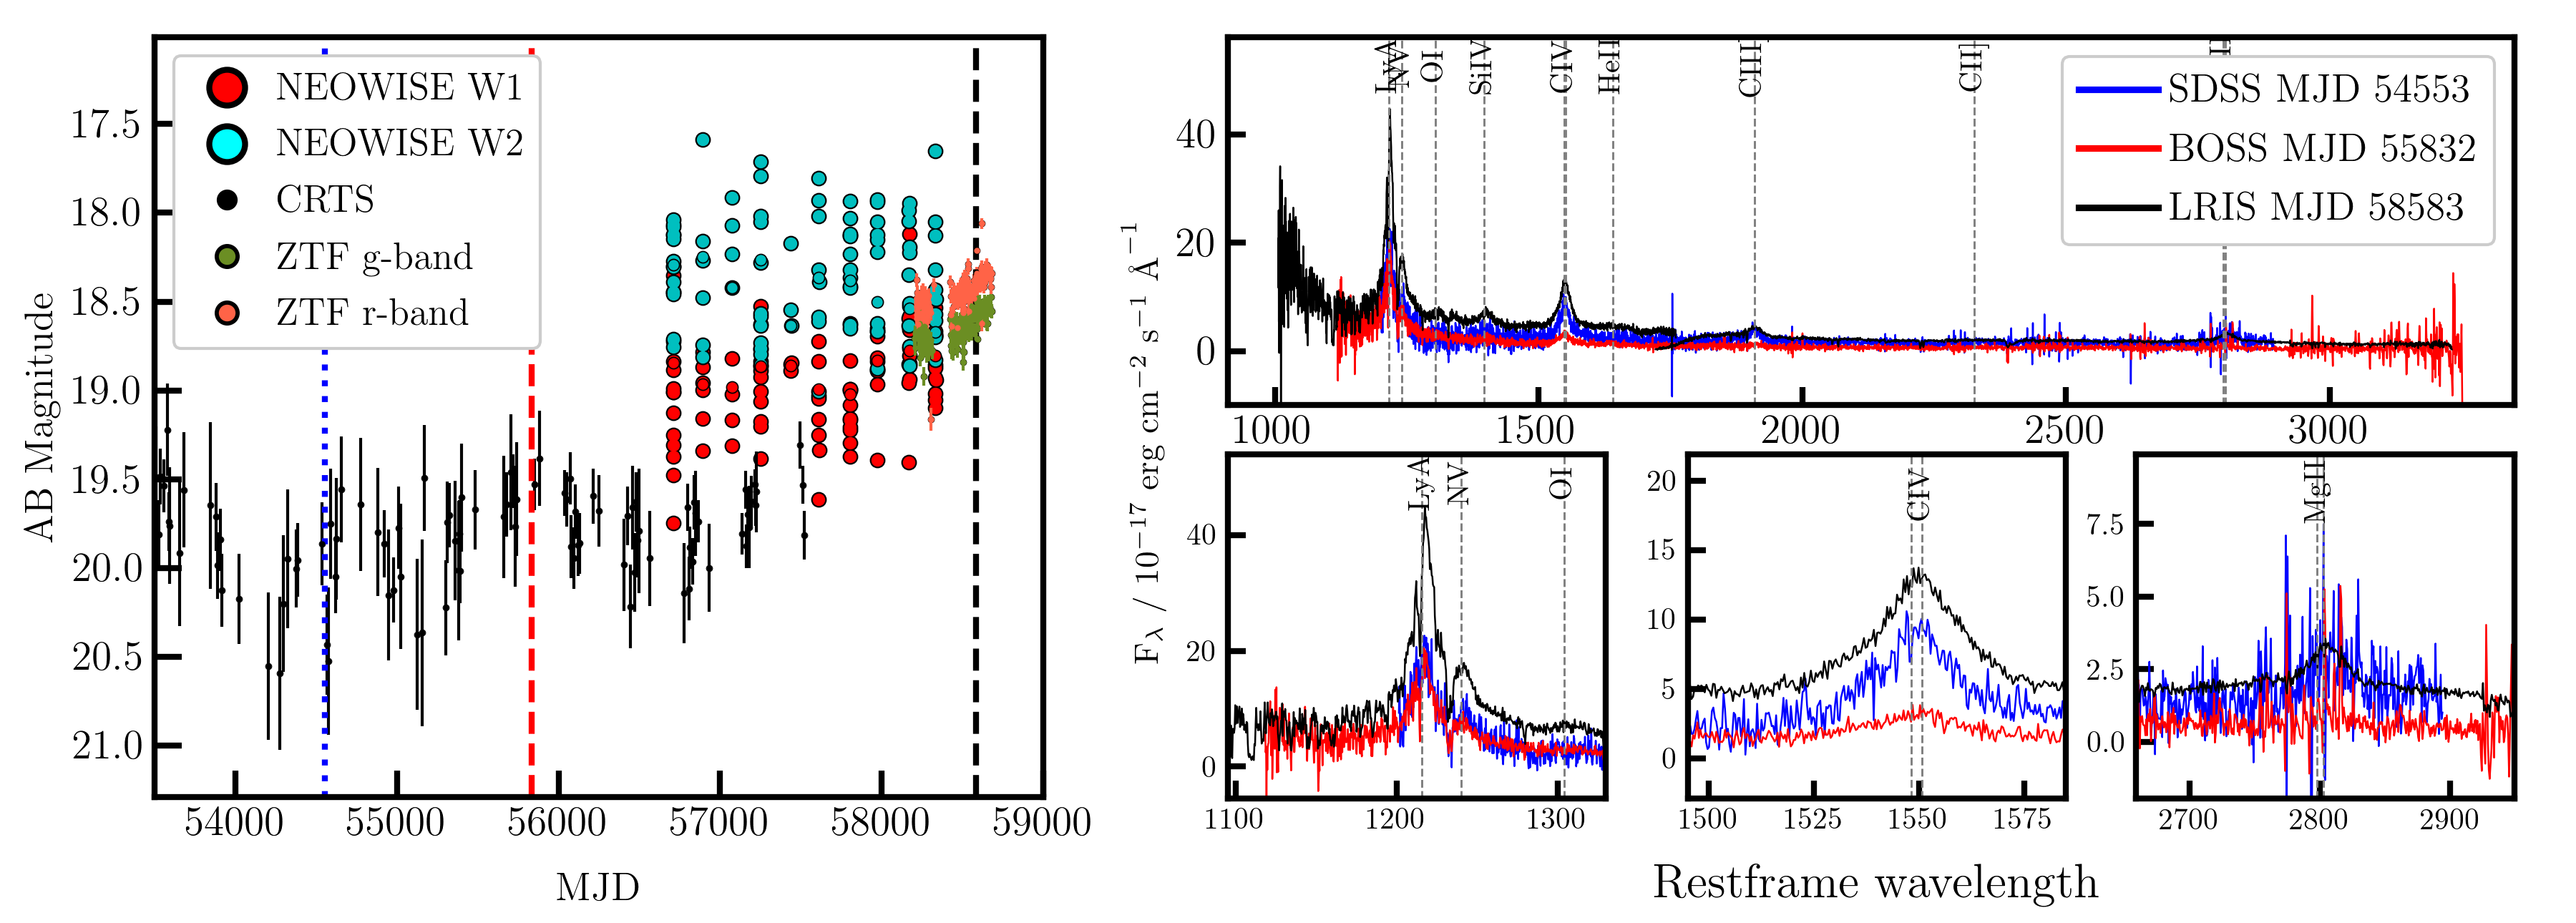
\includegraphics[width=16.7cm, trim=0.0cm 0.1cm 0.2cm 0.1cm, clip]
  {../plots/perObject/J1638+2827_landscape_20190920.png}
  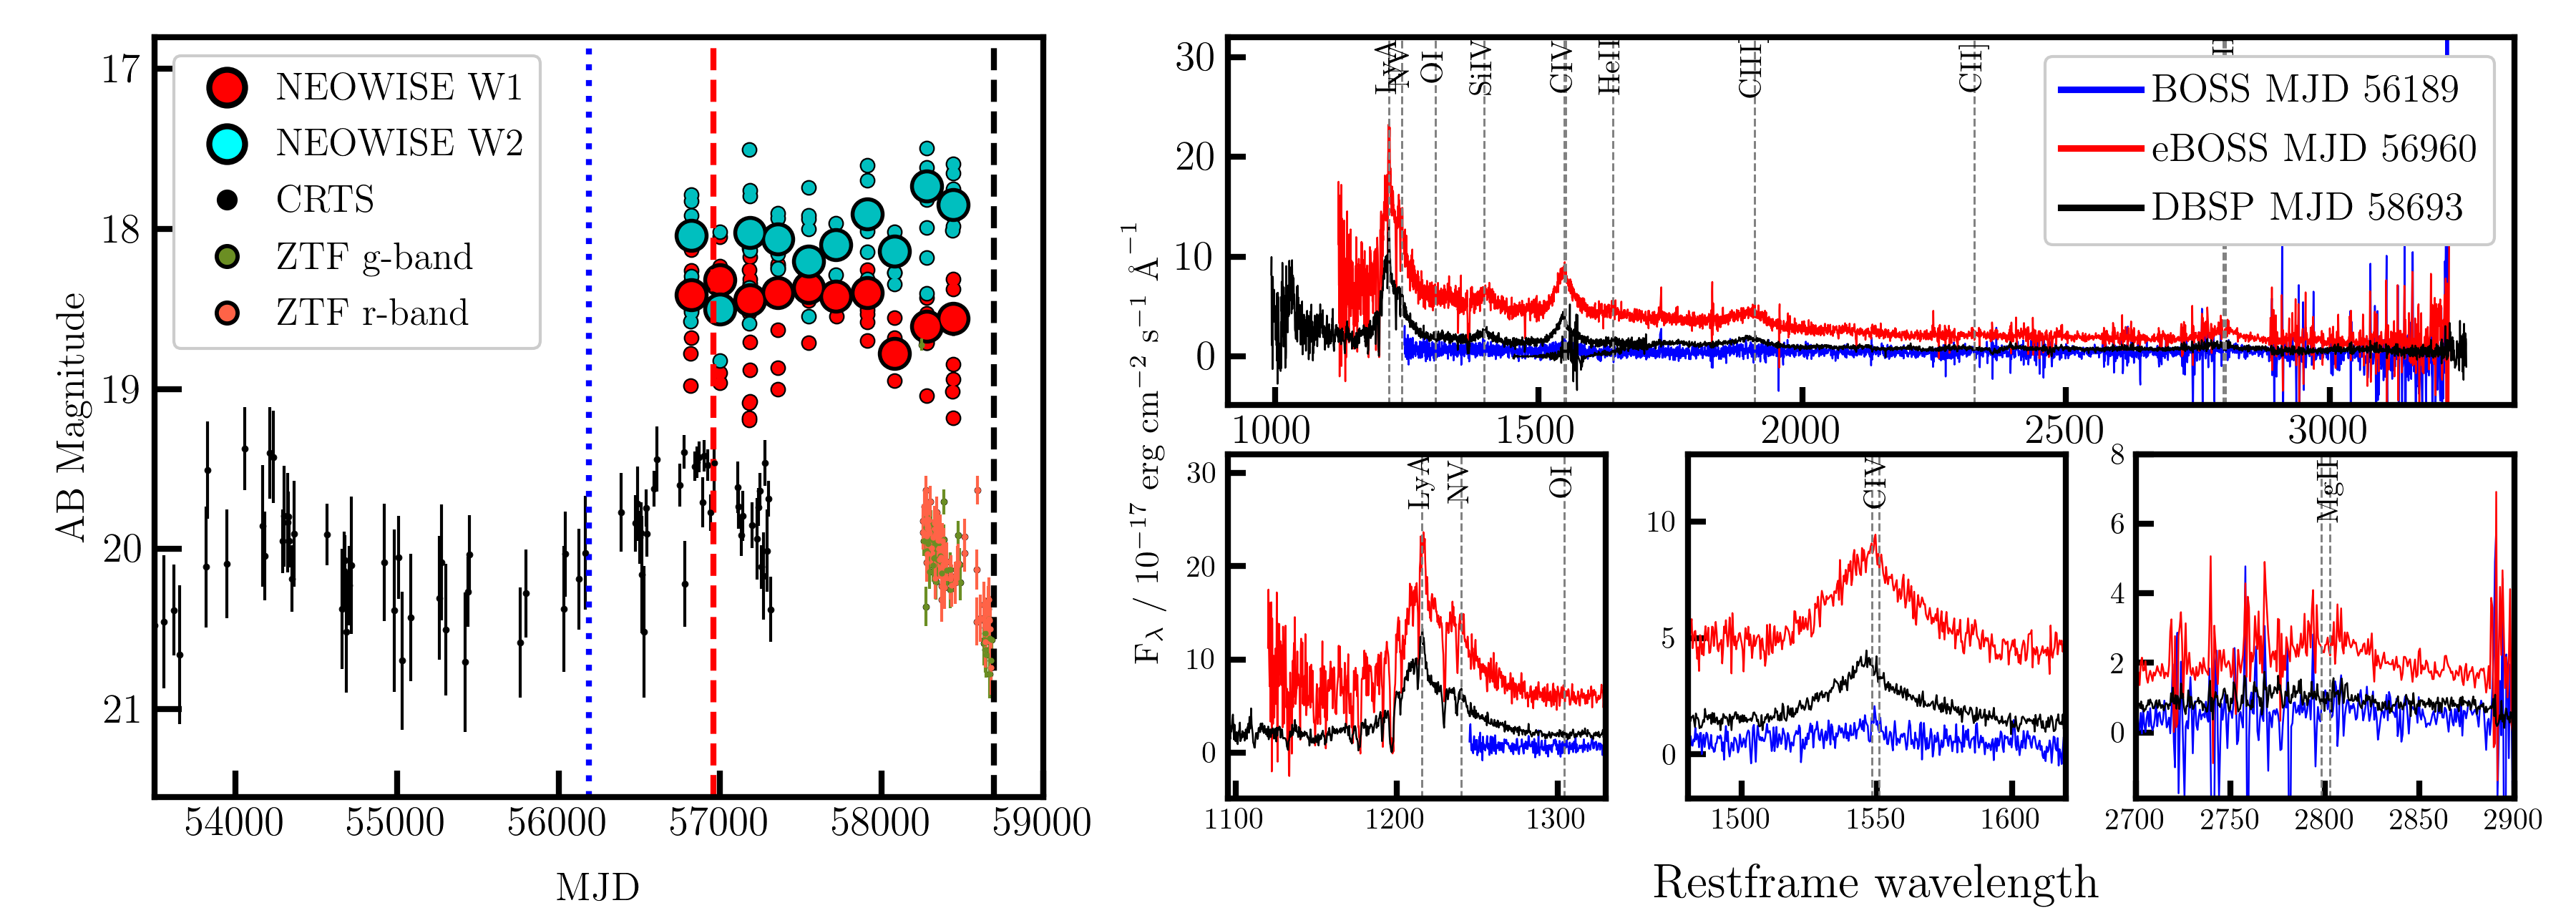
\includegraphics[width=16.7cm, trim=0.0cm 0.1cm 0.2cm 0.1cm, clip]
  {../plots/perObject/J2228+2201_landscape_20190920.png}
  \vspace{-12pt}
  \caption[]{The threes high-$z$ CLQ quasars; 
    SDSS J1205+3422 (top), 
    SDSS J1638+2827 (middle), 
    SDSS J2228+2201 (bottom). 
    % A quasar at $z = 2.2$ with the two spectra showing CIV and CIII] fading.
  }
  \label{fig:civ_clqs2}
\end{figure*}

%%%%%%%%%%%%%%%%%%%%%%%%%%%%%%%%%%%%%%%%%%%%%%%%%%%%%%%%%%%%%%%%%%%%%%%%%%%%%
%%%%%%%%%%%%%%%%%%%%%%%%%%%%%%%%%%%%%%%%%%%%%%%%%%%%%%%%%%%%%%%%%%%%%%%%%%%%%
%%
%%   SECTION 3   SECTION 3   SECTION 3   SECTION 3   SECTION 3   SECTION 3  
%%   SECTION 3   SECTION 3   SECTION 3   SECTION 3   SECTION 3   SECTION 3  
%%   SECTION 3   SECTION 3   SECTION 3   SECTION 3   SECTION 3   SECTION 3  
%%
%%%%%%%%%%%%%%%%%%%%%%%%%%%%%%%%%%%%%%%%%%%%%%%%%%%%%%%%%%%%%%%%%%%%%%%%%%%%%
%%%%%%%%%%%%%%%%%%%%%%%%%%%%%%%%%%%%%%%%%%%%%%%%%%%%%%%%%%%%%%%%%%%%%%%%%%%%%
\section{Results}
Figure~\ref{fig:civ_clqs} presents the threes high-$z$ CLQ quasars. 
%%
%%
For J1638+2827, over the course of 1279 days observed, 400 days in the rest-frame, the  broad \civ and \ciii BEL start to fade.  
For J2228+2201, over the course of 771 days observed, 240 days in the rest-frame, broad \civ and \ciii BELs both emerge and the 
standard UV/blue continuum slope increases in flux. 
the UV/blue continuum diminishes and the shape of \lya changes. 

Nunc semper quam et leo interdum vulputate eu quis magna. Sed nec arcu
at orci egestas convallis. Aenean quam velit, aliquam vitae viverra
in, elementum vel elit. Nunc suscipit aliquet sapien a suscipit. Cras
nulla ipsum, posuere eu fringilla sit amet, dapibus ultricies
nulla. Nullam eu augue id purus mollis dignissim sed et
libero. Phasellus eget justo sed neque pellentesque egestas nec id
arcu. Donec facilisis pulvinar sapien et fringilla. Suspendisse
vestibulum rhoncus sapien id laoreet. Morbi et orci vitae tortor
imperdiet imperdiet. In hac habitasse platea dictumst. Vivamus vel
neque id mi ultrices tristique. Integer quam libero, ornare vel
gravida in, feugiat a ante. Nam dapibus, tellus vitae pellentesque
cursus, dui nisl egestas augue, non fermentum nisl est nec
nisi. Vestibulum nec mi justo, eget dapibus velit.


\begin{figure}
  \centering
  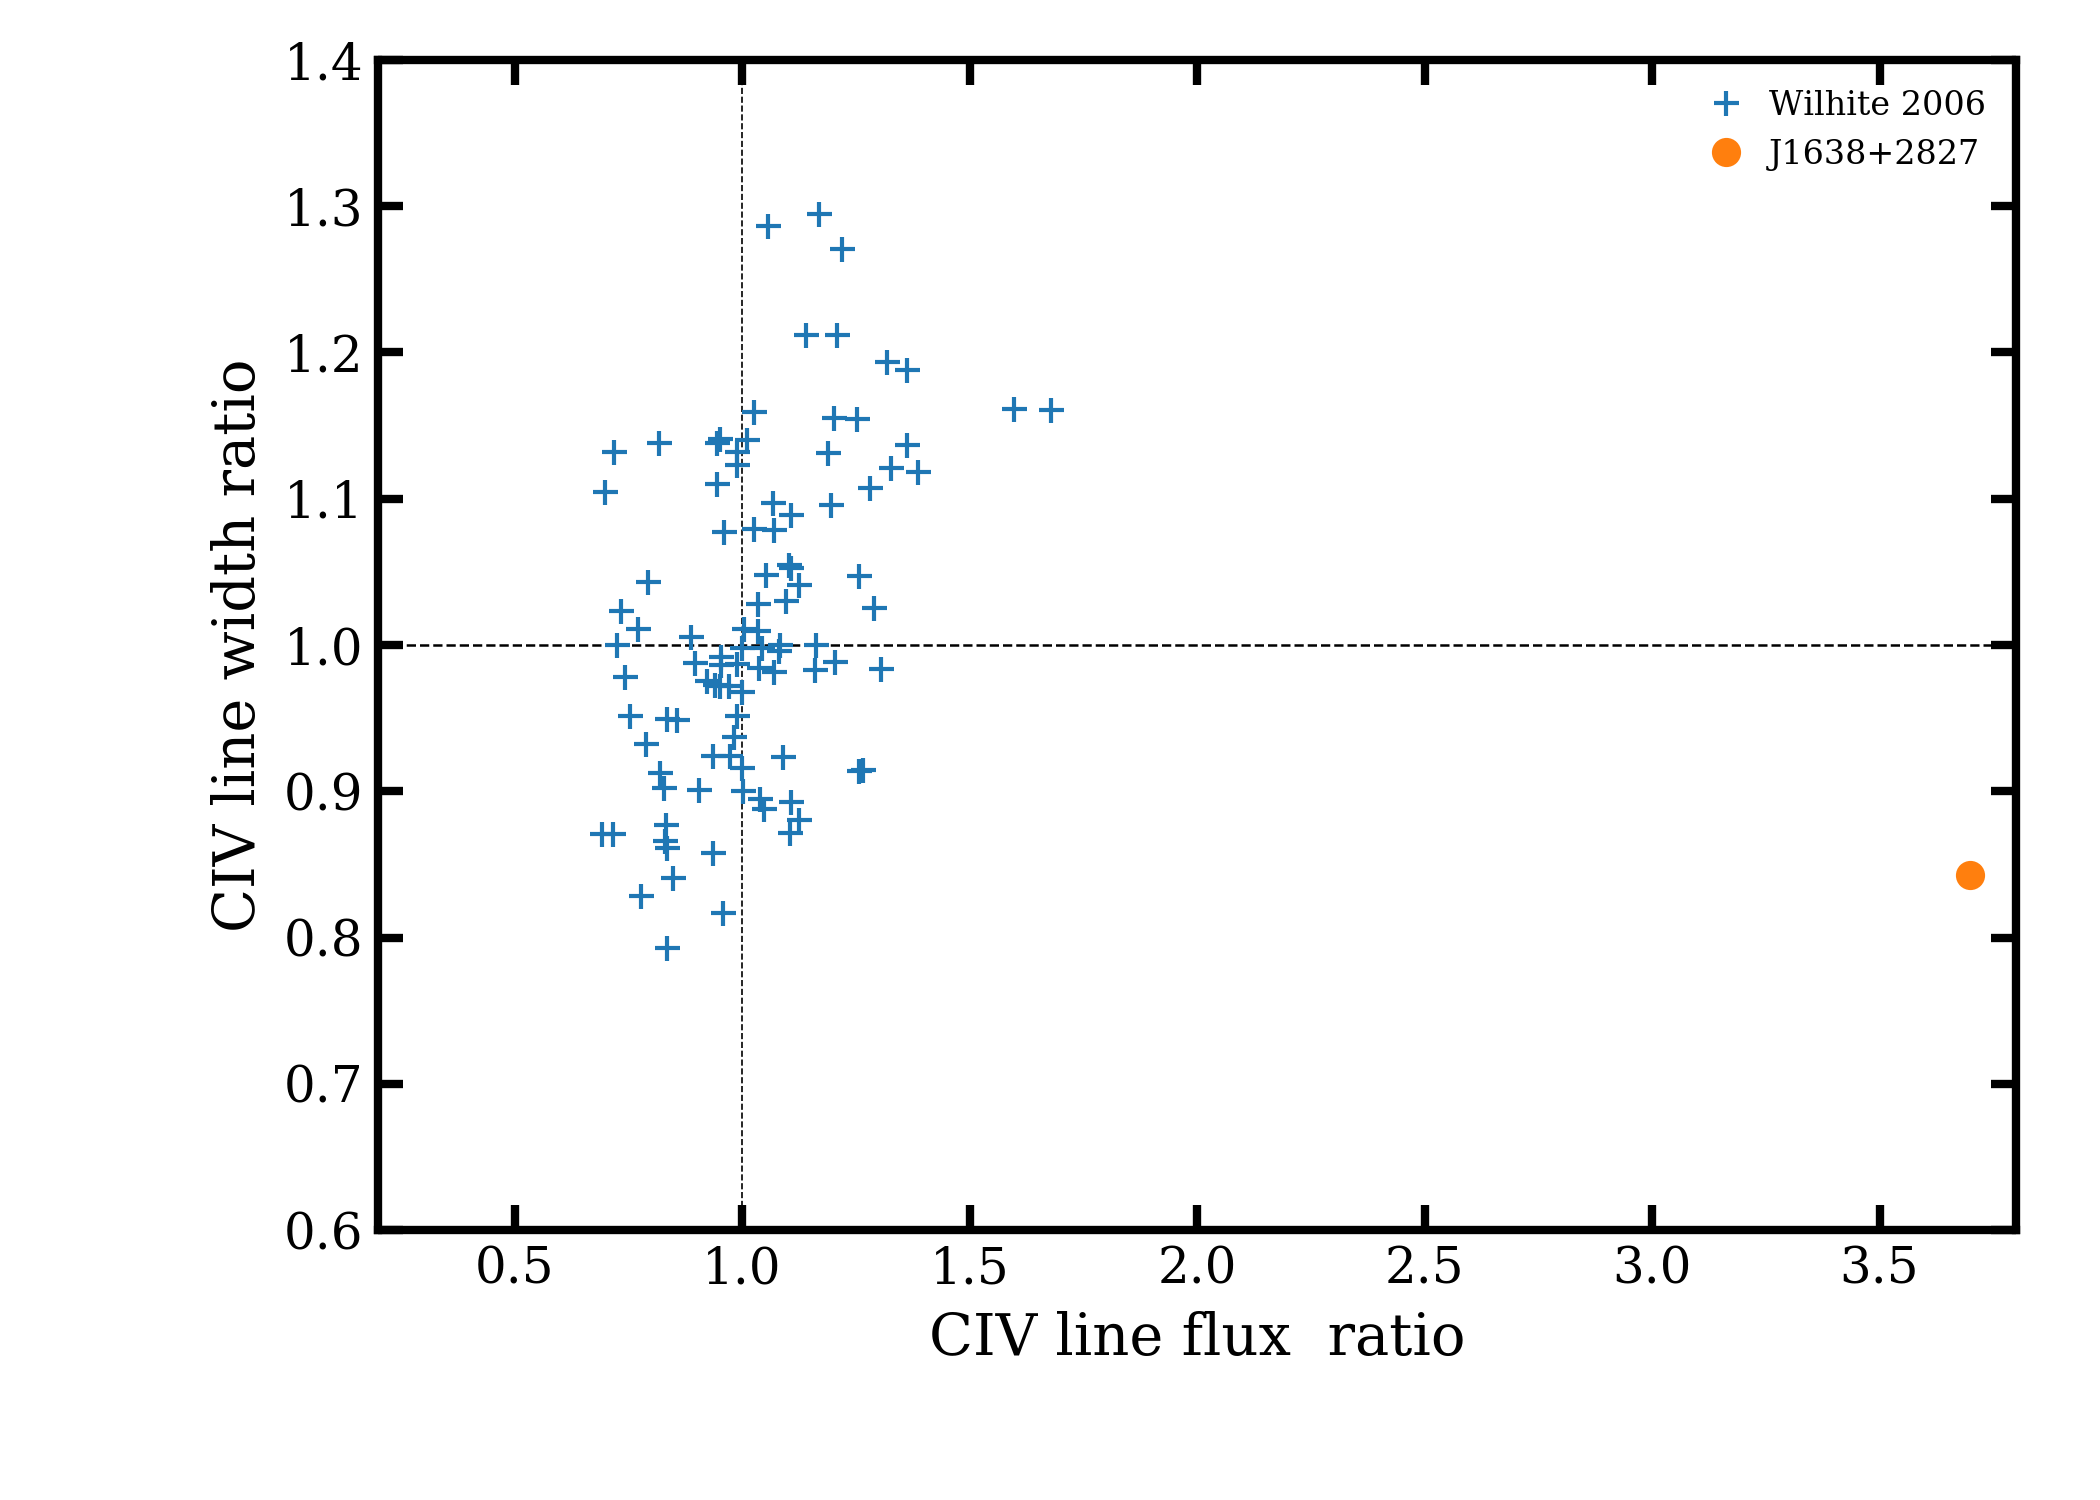
\includegraphics[width=8.7cm, trim=0.2cm 0.2cm 0.2cm 0.2cm, clip]
  {../plots/Wilhite/Wilhite_2006_Fig2_redux_20190830.png}
% {figures/The_3_CIV_CLQs_20190917.pdf}
   \vspace{-12pt}
  \caption[]{
The Change in \civ line width vs. line flux change. 
Data from \citet{Wilhite2006} with a sample of 105 quasars observed at
multiple epochs by the Sloan Digital Sky Survey. We find a strong
correlation between the change in the C iv line flux and the change in
the line width, but no correlations between the change in flux and
changes in line center and skewness.}
  \label{fig:Wilhite2006_comparison}
\end{figure}
From Figure~\ref{fig:Wilhite2006_comparison} there appears to be a
strong correlation between the change in the line flux and the change
in the line width.  Figure~\ref{fig:Wilhite2006_comparison} shows the
epoch-to-epoch flux ratio versus the ratio of line widths.

In the context of CLQs at lower-$z$...  Sociis natoque penatibus et
magnis dis parturient montes, nascetur ridiculus mus. Duis tempus,
lectus nec ultricies mollis, mi orci feugiat nulla, a bibendum velit
orci nec lacus. Duis a odio in nisi egestas dictum. Nullam vel quam
mauris, eget consectetur orci. Morbi ac mi sit amet neque consectetur
tempus ac eget est. Curabitur malesuada arcu sit amet metus dictum at
dapibus arcu accumsan. Fusce sollicitudin luctus rutrum.  Balmer CLQs
vs. \civ CLQs...


\subsection{J1205+3422 }
SDSS J120544.67+342252.4, observed by SDSS, first reported in \citet{Schneider2007}. 
Redshift of $z=$2.068$\pm$0.00027. 
%% targeting_flags	SERENDIP_BLUE QSO_CAP
plate	2089 
mjd	53498
fiberid	427


\subsection{J1638+2827}
SDSS J163852.93+282707.7       16h38m52.9s +28d27m08s  \\
First reported in \citet{Schneider2010}. 
Selected by {\tt SERENDIP\_BLUE} and {\tt QSO\_MAG\_OUTLIER} in SDSS \citep{Richards2002}, meaning...
Selected as a $z>2$ known quasar and passed BOSS quasar target selections \citep{Ross2012}. 


R.A. (J2000) = 249.72058 degs. \\
Decl. (J2000) = 28.45217 degs. \\
\href{skyserver.sdss.org/dr15/en/tools/explore/Summary.aspx?id=1237662301375824232}{SDSS SkyServer} 
All Spectra of this Object:: \\
specObjId	plate	MJD	fiber	ra	dec	redshift \\
5855854441601671168	5201	55832	178	2.186$\pm$0.00073\\
3319321776793610240	2948	54553	614	2.185$\pm$0.00043\\


\subsection{J2228+2201}
SDSS J222818.76+220102.9 (R.A. 337.078194926, Decl. 22.017477924) was first reported in 
\citet{Paris2017}. 

%%\href{https://skyserver.sdss.org/dr12/en/tools/chart/navi.aspx?ra=337.077916666667&dec=22.0173888888889&scale=0.2&width=120&height=120&opt=
\href{skyserver.sdss.org/dr15/en/tools/explore/summary.aspx?id=1237678579819479655}{SDSS SkyServer}
All Spectra of this Object:: \\
specObjId	plate	MJD	fiber	ra	dec	redshift \\
8536790363997708288	7582	56960	790	2.222$\pm$0.00038\\
6888453645991387136	6118	56189	720	2.217$\pm$0.00208\\



%Plate: 2948, MJD: 54553, Fiber: 0614
%https://dr12.sdss.org/spectrumDetail?mjd=54553&fiber=614&plateid=2948

\begin{table*}
  \centering
  \begin{tabular}{l  l  l    lll}
    \hline \hline 
    Line 	    &   Rest	      & Line       & Line	       &	Line			                 &   Continuum \\ 
    Name	    &   Wavelength  &  $z$       & $\sigma$ 	&	Flux			                 & \\
                    &    $\AA $        &              & /  km s$-1$	&     10$^{-17}$ erg/cm$2$/s &  10$^{-17}$ erg/cm$^2$/s/\AA  \\
Ly$\alpha$  &	 1215.7	&	2.186      &	1362	&	510.5		                &	7.224 \\
\nv		    &   1240.8	&	2.184     &	 854.6	&	122.4	                    	&	5.546 \\ 
\civ		    &  1549.5	&	2.184    &	1927	&	462.6		                &	2.722 \\ 
\heii	    &	 1640.4	&	2.184    &	1927	&    	  8.067	                   	&	2.447 \\  
\ciii 	    &	 1908.7	&	2.184    &	1927	&	164.6	                   	&	1.966  \\ 
\mgii	    &	 2800.3	&	2.184   & 	1927	&	187.4	                   	&	1.513  \\
   \hline \hline   
  \end{tabular}
  \caption{Line Measurement Information}
 \label{tab:line_values}
\end{table*}



\begin{table*}
  \centering
  \begin{tabular}{l  lll lll  }
    \hline \hline 
                                    &                               &                                           &                                                      &                                  &                         & \\  
                                  \multicolumn{7}{c}{J1638+2827}  \\
                                    &                               &                                           &                                                      &                                  &                         & \\  
   \hline                       
%                                   &                               &                                           &                                                      &                                  &                         & \\  
    Line      	             & Line  $\sigma$     & Line  Flux                           &   Continuum                                 & Line  $\sigma$          & Line  Flux        &   Continuum                                    \\
%    Wavelength	             & /  km s$^{-1}$         &   10$^{-17}$ erg/cm$2$/s  & 10$^{-17}$ erg/cm$^2$/s/\AA      &  /  km s$-1$             & / 10$^{-17}$ erg/cm$2$/s   & /10$^{-17}$ erg/cm$^2$/s/\AA       \\
                                     & \multicolumn{3}{l}{MJD 54553}                                                                                   & \multicolumn{3}{l}{MJD 55832}                                                                                                          \\
    Ly$\alpha$1215.7    &  1362	            &	510.5		                  &	7.224                                           &  1769	                &   633.9	              &  5.376     \\
    \nv1240.8	            &   854.6	            &	122.4	                    	  &	5.546                                           & 1012	                &  107.1		      &  4.645\\ 
    \civ1549.5         	    &	 1927	            &	462.6		                  &	2.722                                           & 2287	                &  125.1		      &  1.256      \\  
    \heii1640.4	            &	 1927    	            &      8.067	                   	  &	2.447                                           & 2287	                &    10.68	      &  1.001\\  
    \ciii1908.7        	    &	 1927	            &	164.6	                   	  &	1.966                                          & 2287	 	                &     29.53	      &  0.6008\\ 
    \mgii2800.3	    &   1927	            &	187.4	                   	  &	1.513                                          & 2287 	 	         &    34.66	      &  0.3461  \\
                                    &                               &                                           &                                                      &                                  &                           &                \\  
   \hline \hline   
  \end{tabular}
  \caption{Line Measurement Information. 
    Line $\sigma$ in units of   km s$-1$; 
    Line flux          in units of  10$^{-17}$ erg/cm$^2$/s; 
    Continuum      in units of  10$^{-17}$ erg/cm$^2$/s/ \AA; 
}
 \label{tab:line_values}
\end{table*}

%Plate: 5201, MJD: 55832, Fiber: 178
%https://dr12.sdss.org/spectrumDetail?mjd=55832&fiber=178&plateid=5201

%Line		Rest		        Line	        Line		        Line			   Continuum
%Name		Wavelength	z	        sigma 		Flux	
%                       [Å]			               [km s-1]  	[10-17erg/cm2/s] 	   [10-17erg/cm2/s/Å]
%Ly_alpha	1215.7		2.186	1769		633.9		   5.376
%N_V		1240.8		2.185	1012		107.1		   4.645
%C_IV		1549.5		2.185	2287		125.1		   1.256
%He_II		1640.4		2.185	2287		 10.68		   1.001
%C_III]		1908.7		2.185	2287	 	 29.53		   0.6008
%Mg_II		2800.3		2.185	2287 	 	 34.66		   0.3461

%So, ratios, MJD 54553 / MJD 55832::
%$Ly_alpha	1215.7		—	0.770		0.805			1.344			
%N_V		1240.8		—	0.844		1.143			1.194
%C_IV		1549.5		—	0.843		3.698			2.167			
%He_II		1640.4		—	0.843		0.755			2.445			
%C_III]		1908.7		—	0.843		5.574			3.27			
%Mg_II		2800.3		—	0.843		5.407			4.37





%%%%%%%%%%%%%%%%%%%%%%%%%%%%%%%%%%%%%%%%%%%%%%%%%%%%%%%%%%%%%%%%%%%%%%%%%%%%%
%%%%%%%%%%%%%%%%%%%%%%%%%%%%%%%%%%%%%%%%%%%%%%%%%%%%%%%%%%%%%%%%%%%%%%%%%%%%%
%%
%%   SECTION 4   SECTION 4   SECTION 4   SECTION 4   SECTION 4   SECTION 4  
%%   SECTION 4   SECTION 4   SECTION 4   SECTION 4   SECTION 4   SECTION 4  
%%   SECTION 4   SECTION 4   SECTION 4   SECTION 4   SECTION 4   SECTION 4  
%%
%%%%%%%%%%%%%%%%%%%%%%%%%%%%%%%%%%%%%%%%%%%%%%%%%%%%%%%%%%%%%%%%%%%%%%%%%%%%%
%%%%%%%%%%%%%%%%%%%%%%%%%%%%%%%%%%%%%%%%%%%%%%%%%%%%%%%%%%%%%%%%%%%%%%%%%%%%%
\section{Discussion and Conclusions}
Lorem ipsum dolor sit amet, consectetur adipiscing elit. Aliquam porta
sodales est, vel cursus risus porta non. Vivamus vel pretium
velit. Sed fringilla suscipit felis, nec iaculis lacus convallis
ac. Fusce pellentesque condimentum dolor, quis vehicula tortor
hendrerit sed. Class aptent taciti sociosqu ad litora torquent per
conubia nostra, per inceptos himenaeos. Etiam interdum tristique diam
eu blandit. Donec in lacinia libero.

Sed elit massa, eleifend non sodales a, commodo ut felis. Sed id
pretium felis. Vestibulum et turpis vitae quam aliquam convallis. Sed
id ligula eu nulla ultrices tempus. Phasellus mattis erat quis metus
dignissim malesuada. Nulla tincidunt quam volutpat nibh facilisis
euismod. Cras vel auctor neque. Nam quis diam risus.

Nunc semper quam et leo interdum vulputate eu quis magna. Sed nec arcu
at orci egestas convallis. Aenean quam velit, aliquam vitae viverra
in, elementum vel elit. Nunc suscipit aliquet sapien a suscipit. Cras
nulla ipsum, posuere eu fringilla sit amet, dapibus ultricies
nulla. Nullam eu augue id purus mollis dignissim sed et
libero. Phasellus eget justo sed neque pellentesque egestas nec id
arcu. Donec facilisis pulvinar sapien et fringilla. Suspendisse
vestibulum rhoncus sapien id laoreet. Morbi et orci vitae tortor
imperdiet imperdiet. In hac habitasse platea dictumst. Vivamus vel
neque id mi ultrices tristique. Integer quam libero, ornare vel
gravida in, feugiat a ante. Nam dapibus, tellus vitae pellentesque
cursus, dui nisl egestas augue, non fermentum nisl est nec
nisi. Vestibulum nec mi justo, eget dapibus velit.

Cras in laoreet mauris. Vivamus nec nulla a dui commodo
adipiscing. Proin vulputate lectus nec arcu iaculis sit amet auctor
ligula ultricies. Phasellus condimentum gravida tincidunt. Phasellus
et mauris ac nibh vestibulum vehicula. Morbi et augue id purus gravida
sagittis quis in sem. Phasellus quis risus bibendum eros luctus
auctor.

Etiam mollis viverra nisi eget aliquet. Aliquam erat volutpat. Vivamus
tristique, nisl eu malesuada semper, libero tortor convallis elit, a
scelerisque orci nisi lacinia turpis. In lacinia ultrices
volutpat. Proin ultrices luctus tellus, in placerat eros tincidunt
id. Ut varius iaculis quam in consequat. Nulla nec orci est, sit amet
pellentesque nisl. Mauris non cursus lectus. Praesent placerat leo vel
erat gravida lacinia. Donec vehicula consectetur lectus vitae
luctus. Praesent nisl justo, laoreet elementum facilisis vel,
tristique ac enim. Etiam vel quam ut quam eleifend
tincidunt. Suspendisse sit amet eros vel elit ullamcorper
laoreet. Etiam venenatis sodales turpis, nec lacinia ligula hendrerit
nec. Nam eu vulputate purus. Quisque facilisis congue metus, sed
imperdiet lorem rhoncus sit amet.

In this paper we have... 
\begin{itemize}
\item Pellentesque vel elit neque, in interdum lacus. Quisque sodales, nunc et luctus convallis, nisl dui luctus dui, at congue urna velit a; 
\item At sit amet sapien a risus dapibus sagittis. Cras sed ultricies erat. Donec id metus sed urna lacinia convallis vel sed enim. 
\item Nisi libero, ornare vel bibendum eu, sollicitudin sed leo. Cras tincidunt aliquet ultricies. Cras pretium velit leo, in malesuada. 
\item Duis sagittis ultricies interdum. Proin sit amet sem nec metus feugiat pharetra.
\end{itemize}

Aliquam ac metus nec odio tempus pharetra sed nec diam. Sed eget arcu
nulla. Etiam elementum ultrices ligula, at iaculis libero feugiat
bibendum. Suspendisse potenti. Nam pharetra adipiscing
euismod. Quisque imperdiet dignissim odio, sed volutpat justo
tincidunt eu. Nunc vehicula pharetra suscipit. Integer aliquet pretium
ipsum vel ultrices. Nam rutrum nibh ac quam pulvinar molestie.

Sed sed ipsum diam. In risus tortor, sagittis eu auctor in, varius in
dui. Mauris a nunc ut ligula ullamcorper tincidunt. Nunc aliquam eros
ac risus pellentesque aliquam. Phasellus augue velit, varius at
porttitor sit amet, pretium eget felis. Ut mollis tellus elementum
magna porttitor rutrum. Etiam blandit leo eget est consectetur
imperdiet. Quisque et diam nec orci vulputate varius vitae id sapien.


\bibliographystyle{mnras}
\bibliography{tester_mnras}


% Don't change these lines
\bsp	% typesetting comment
\label{lastpage}
\end{document}


\end{document}